\chapter{绪\hskip 0.4cm 论}
\label{chap1}
\section{研究背景}
	\textbf{能量信息物理融合系统}
	
	信息物理融合系统(Cyber-Physical Systems,CPS)\citep{谭朋柳2017面向医疗的,lee2011introduction}是一种综合了计算、网络和物理环境的多维复杂系统,它通过计算、通信和控制技术的有机融合与深度协作,实现大型工程系统的实时感知、动态控制和信息服务。
	
	现今,人们对能源的需求处于高速增长中。各个国家尤其是像我国这样的发展中国家为了发展经济,存在大量的能源需求。目前,人类约$80\%$的能源都是从煤炭、石油和天然气中获得,并且预计在接下来的二十年中,能源的需求量还将増长约一半。然而,地球资源是有限的,日益增长的能源需求与资源有限的现状引发了人们对能源危机(Energy Crisis)爆发的担忧,系统能耗越来越受到学术界和工业界的重视。
	能量信息物理融合系统(Cyber-Physical Energy System,CPES)\citep{Van2017Cyber,DBLP:journals/corr/StamatescuSACF16}——一种结合了网络基础设施与物理基础设施来对能量进行有效管理和控制的现代能量系统应运而生。除了密切关注系统能耗外,与CPS相同,CPES存在于复杂的物理环境中,与外界的各种随机行为存在交互,且系统中连续行为和离散行为共存,因此,系统具有随机和混成的特点。更高级的CPES控制器设计不仅要求能够节约系统的整体能耗,而且会要求保证一定的服务质量\citep{DBLP:conf/compsac/ChenGCDLS15}。
	
	\textbf{智能建筑}
	
	智能建筑(Smart Building)\citep{Kleissl2010Cyber,DBLP:conf/wsc/OckIF16}作为智能电网(Smart Grid)技术\citep{Jacobsen2015Smart}的重要组成部分逐渐在国内外兴起。智能建筑是一种典型的嵌入式传感和网络信息处理深度耦合的CPES,它与外界环境——包括物理环境和用户进行频繁交互,并利用调度器对功能构件实行智能控制,在节约能耗的基础上为人类提供适宜的室内环境,是新一代建筑设计的趋势。据调查统计,建筑相关能耗已占全社会总体能耗的$47\%$\citep{DBLP:conf/smartgreens/LiTTYW17},解决能源成本上升问题、确保环境可持续性,降低新建筑物和现有建筑物的能源消耗已成为所有利益攸关者——包括政府、建筑开发商、业主、经营者、租户和用户的迫切需求。
	由于人们大部分时间都是在建筑物中度过的,一个健康又舒适的环境对于人类生活和社会生产力来说是至关重要的。智能建筑通过智能控制保证了人们生活的舒适性、安全性和效率,其系统设计具有重要意义。
	%智能建筑需要对灵活的能源需求和异构的能源实现合理调度,从而节约能源总成本。根据所有收集的信息,建筑管理系统控制从不同能源到各种功能构件的能量流。
	
	%Intelligent buildings are becoming a trend of the next-generation‘s buildings, which facilitate intelligent control of the building to satisfy the changing needs effectively. Since people spend 80% of their lifetime in buildings, a healthy and comfortable environment is important for occupants‘ well-being and productivity [1]. Intelligent buildings promote occupants‘ wellbeing, safety, productivity, and building‘s sustainability through intelligent technologies

\section{研究现状}	
	%CPS:A cyber-physical system (CPS) is a mechanism controlled or monitored by computer-based algorithms, tightly integrated with the internet and its users. In cyber-physical systems, physical and software components are deeply intertwined, each operating on different spatial and temporal scales, exhibiting multiple and distinct behavioral modalities, and interacting with each other in a myriad of ways that change with context.[1] Examples of CPS include smart grid, autonomous automobile systems, medical monitoring, process control systems, robotics systems, and automatic pilot avionics.[2]

	%CPS involves transdisciplinary approaches, merging theory of cybernetics, mechatronics, design and process science.[3][4][5] The process control is often referred to as embedded systems. In embedded systems the emphasis tends to be more on the computational elements, and less on an intense link between the computational and physical elements. CPS is also similar to the Internet of Things (IoT) sharing the same basic architecture, nevertheless, CPS presents a higher combination and coordination between physical and computational elements.[6]
	
	%信息物理融合系统(Cyber-Physical Systems, CPS)的一个重要应用领域就是能量系统。当下大多数的能量系统需要管理物理和计算机变量,譬如电池寿命、功率通量、计算过程和网络限制。并且这些系统往往具有多层和分布式的架构。为了让未来的能量系统适应这些挑战,这些系统需要具备自适应的功能,譬如
	
	%Since dealing with the uncertainties of environment in an early stage can enhance the probability of a successful implementation in a cost-effective manner, there are many research works presented to handle the uncertainties of environment during the requirement phase[5]–[7].
	%In summary, the following open issues have been identified and need to be addressed in future research and development [3,6,7,12,25]:
	%– A cyber-physical, multi-domain approach for analysing and validating CPES on the system level is missing today; existing methods are mainly focusing on the component level 
	%- system integration topics including analysis and evaluation are not yet addressed in a holistic manner.
	%- A holistic validation framework (incl. analysis and evaluation/benchmark criteria) and the corresponding RI with proper methods and tools needs to be developed.
	%– Harmonized and standardized evaluation procedures need to be developed.
	%– Well-educated professionals, engineers and researchers that understand smart grid systems in a cyber-physical manner need to be trained on a broad scale.
	%总结来说,在将来的研究和发展中,下列这些开放性问题需要被重视和发展:
	%一个信息物理融合的、多领域的从系统层级验证CPES方法如今尚未存在,现有的方法只是关注在构件层面;
	%系统的综合性问题,诸如分析和评估还没有一个综合的处理方法;	
	%具有丰富经验的专家、工程师和研究人员
	能量信息物理融合系统包含了物理变量和信息技术变量,诸如电池寿命、功率、计算过程和网络限制等。由于能量利用率在CPES的设计中起着重要影响,目前为止,大部分的研究都关注在系统的能耗方面。例如,在\citep{DBLP:journals/pieee/Ilic07}中,Marija等学者基于微分代数等式(Differential Algebraic Equations, DAE)提出了一个建模电力系统的通用方法。他们所提的基于DAE的模型被时间间隔简化和分割,以捕捉感兴趣的系统行为;在\citep{DBLP:journals/tsmc/IlicXKM10}中,Ilic等学者提出了一种针对未来CPES的动态模型,模型背后的数学描述是物理环境相关的计算机技术。	
	%然而,上述的这些研究都仅仅局限于系统的建模与描述,并未提供一个针对CPES的从需求分析、到模型设计和模型验证的完整建模方法。
	
	而关于智能建筑的建模与分析,国内外许多学者也已经做出了诸多研究贡献。在 \citep{DBLP:journals/chinaf/DavidDLMS12}中,Alexandre David等学者提出了利用统计模型检测技术分析能耗感知建筑的框架。他们利用基于蒙特卡洛模拟的统计模型检测技术,在模型验证工具UPPAAL-SMC中构建了智能建筑不同模块对应的模板,实现了对系统特定性质的高效验证;
	在\citep{不确定环境下智能大厦空调系统调度策略评估}中,陈铭松等学者针对智能建筑中空调的调度问题,设计了不同的调度策略,并分析不同策略下用户的舒适度和大厦的能耗;
	陈小红等学者在\citep{DBLP:conf/compsac/ChenGCDLS15}中给出了一种基于环境本体的能量信息物理融合系统的分析方法,将系统元素分为环境和控制器两类,给出了环境本体的自动机模板和利用上下文图构建控制器模型的方法;
	在智能建筑的能耗评估方面,Mendes等学者\citep{Mendes2001Building}提出了一种数学模型并将其应用于建筑的热分析和控制系统设计,用集中式方法建立了房间空气温度模型和建筑围栏多层模型,对室内空气温度进行瞬时分析。他们使用MATLAB/Simulink作为支持工具设计智能建筑的控制系统,对智能大厦进行热性能分析。

	然而,以上的研究都是研究人员基于自身的专业知识,直接构建系统的可执行模型,进而实现模型的验证和分析。这种形式化的方法逻辑严谨、理论性较强,但不利于系统研发人员的学习和理解,在实际应用中,会给项目组成员的沟通带来困扰。
	因此,提供一种从需求出发,将设计模型和可执行的形式化模型相结合的方法是必要的。这种方式不仅有利于研究者之间的交流与沟通,且能够实现模型的属性验证,从而保证系统模型的质量。
	
\section{相关理论与技术}
	\textbf{本体论}

	本体(Ontology)的概念起源于哲学,它是一个解释客观存在系统的抽象本质的哲学术语,它提供了一个分类体系,且这个体系不依赖任何特定的语言。上个世纪80年代,本体概念从哲学领域被引领到计算机领域,并和知识工程信息技术相结合延伸到了人工智能领域(Artificial Intelligence,AI)\citep{王向前2016本体研究综述}。人工智能领域的学者Neches赋予其新的定义,即:本体是构成相关领域词汇的基本术语和关系,以及利用这些术语和关系构成的规定这些词汇外延的规则的定义。经过时间的发展,虽然本体的定义在发生演变,但其概念的定义均包括四个最基础特点:概念化、明确化、形式化和共享化。

	根据本体对领域的依赖程度,可将本体细分为顶级(Top-level)、领域(Domain)、任务(Task)和应用(Application)四类。其中,领域本体(Domain Ontology)的目标是捕获相关的领域知识,确定该领域内共同认可的概念,并从不同层次的形式化模型上给出这些概念和概念之间相互关系的明确定义,提供该领域中发生的活动以及主要理论和基本原理。
	
	近些年,本体论被本广泛应用于不同学科和领域,并已经产出了一些显著的成果:在化学领域,Plinius Ontology\citep{Vet1994The}是关于陶瓷物质化学成分的本体,Chemical-Elements\citep{L1999Building}是关于化学元素周期表的本体;在知识领域,已经成熟的本体包括SENSUS\citep{Cranor2002Sensus}、WordNet\citep{Fellbaum1998WordNet}、CYC\citep{Cranor2002Sensus}等。除此之外,我国近几年也出现了如知网、国共合作历史领域本体等。
	
\textbf{MARTE与UML}

	模型驱动式开发(Model Driven Develoment, MDD)是一种以模型为中心,根据不同抽象层次或视图构造不同模型的开发方法。MDD可以有效控制系统的复杂度,保证系统质量,同时,也是提高系统开发复用性的重要手段。统一建模语言(Unified Modeling Language,UML)\citep{博什2001UML}是支持MDD的常用建模语言之一,它始于1997年的一个OMG(Object Management Group)标准,是一种支持模型化系统开发的图形化语言。UML为开发的所有阶段提供了模型化和可视化支持,包括由需求分析到规格、构造和配置。它基于面向对象的思想,支持系统的多视图建模,其主要模型包括:用例图、类图、活动图、状态图、顺序图、部署图等。
	
	UML的profile是一个包含了为特定领域和目的定制的模型元素的衍型(stereotype)包,它利用衍型、标记值(tagged-value)和约束(constraint)等元素来扩展模型。其中,衍型用于扩展UML的词汇,以创建新的构造块;标记值扩展了UML衍型的特性,用来详细描述衍型的性质和定义等信息;约束则通过增加新的规则或修改现有的规则,扩展了UML的语义。

	MARTE\citep{DBLP:conf/icteri/Mallet13, DBLP:conf/ACISicis/LouatiBDS12} 作为UML的一个重要profile,提供了对实时嵌入式系统建模的诸多规范,并利用值描述语言(Value Specification Language, VSL)来描述UML模型的非功能属性。MARTE主要包括基础模型包、设计模型包和分析模型包三个部分。

	基础模型包主要定义了实时和嵌入式系统中的基本概念,如优先级、响应时间、执行周期和受限资源等。基础模型包中的许多基本概念都在设计和分析模型包被复用,是对系统进行设计和分析的基础,因此也是规范中的核心部分;

	设计模型包提供了具有较高抽象级别的建模元素,用来对实时和嵌入式系统中的并发行为和实时活动主体进行建模,如具有独立控制能力的实时功能模块、受限资源保护模块以及响应并发或实时调用的服务和动作等;

	分析模型包封装了用于分析系统的性能和可靠性的建模元素,如能量消耗、内存占用以及系统的可用性、可靠性和安全性等。
	
\textbf{随机混成自动机}

	虽然UML结合MARTE等profile能够增强领域建模能力,但是,由于其半形式化的特性,MARTE/UML模型不能够实现系统属性的验证和分析。而自动机是一种应用广泛的系统模型,它不仅可以描述系统的动态特性,而且已存在众多基于自动机的模型检测(Model Checking)\citep{Clarke1997Model}方法,可以实现对系统模型的定性、定量分析。
	
	随机混成自动机\citep{Hu2000Towards,David2011Statistical,程贝2016基于抽象和学习的统计模型检测研究}(Stochastic hybrid automata, SHA)是混成自动机加入了随机语义的扩展版本,它的主要元素为位置和迁移。SHA的随机语义主要体现在两方面:1)系统位置之间的迁移可定义离散的概率分布;2)系统位置上可定义停留时间的概率分布。随机混成自动机能够准确地建模混成系统中的随机行为。
	
	UPPAAL\citep{DBLP:journals/spe/BehrmannDLPY11} 是一个针对实时系统的建模、验证集成工具,它将系统定义为时间自动机网络,并扩展了其数据类型。UPPAAL-SMC\citep{DBLP:journals/spe/BehrmannDLPY11,DBLP:journals/corr/abs-1207-1272}是UPPAAL系列工具中利用统计模型检测(Statistical Model Checking, SMC)进行模型验证的工具,其理论基础为随机混成自动机。SMC主要使用统计方法分析复杂系统的模拟执行路径,优点是效率高、执行速度快,该项技术的关键点在于:首先,对仿真产生的系统模拟路径进行伯努利实验,判断模拟路径是否满足给定的系统约束;其次,对模拟路径的样本空间进行统计分析,评估系统满足属性的概率区间。因此,使用UPPAAL-SMC能够实现基于随机混成自动机模型的系统属性分析。

\section{本文工作与主要贡献}	
	智能建筑等CPES融合了不同学科的知识,且系统具有混成和随机的特点,是一种复杂系统。对于这类系统的开发,使用MDD方法至关重要。由国内外研究现状的分析可知,针对智能建筑,现有的建模方法大多直接给出系统的可执行模型,再对模型进行验证、分析。可执行模型抽象程度较高,不利于系统设计、研发人员之间的交流,因此,设计模型和可执行模型相结合的建模方式具有重要意义。这种方式又引入了两个新问题:1)如何根据需求从复杂的CPES系统中确定建模元素,指导建模系统设计模型?2)如何将设计模型和可执行模型连接起来?基于MDD的思想,本文提出了一种智能建筑能耗的建模与分析方法,并解决了上述问题。
	%文献\citep{博什2001UML}中指出了,建模的原因是“不能完整地理解一个复杂系统”。对系统建模不仅有助于按照实际情况或所需的样式对系统进行可视化,而且能够规约系统的结构和行为、指导构建系统的模板。基于MDD的思想,
	
	
	%首先,提供一种从系统需求来明确建模的元素,及它们之间关系方法。接着,通过预先的分析指导建模MARTE/UML多视图模型,便于不同研究者之间的交流、沟通。为了实现系统模型的定性、定量分析,还需要特定技术将设计模型转换为可执行模型,在保证转换正确性的前提下,完成系统的分析、验证。
	
	%如图\ref{approach-framework}所示,针对智能建筑这一典型的CPES系统,给出了一个对其进行需求分析、模型设计到模型验证的完整方法。
	
	\begin{figure}[!t]
	\centering
	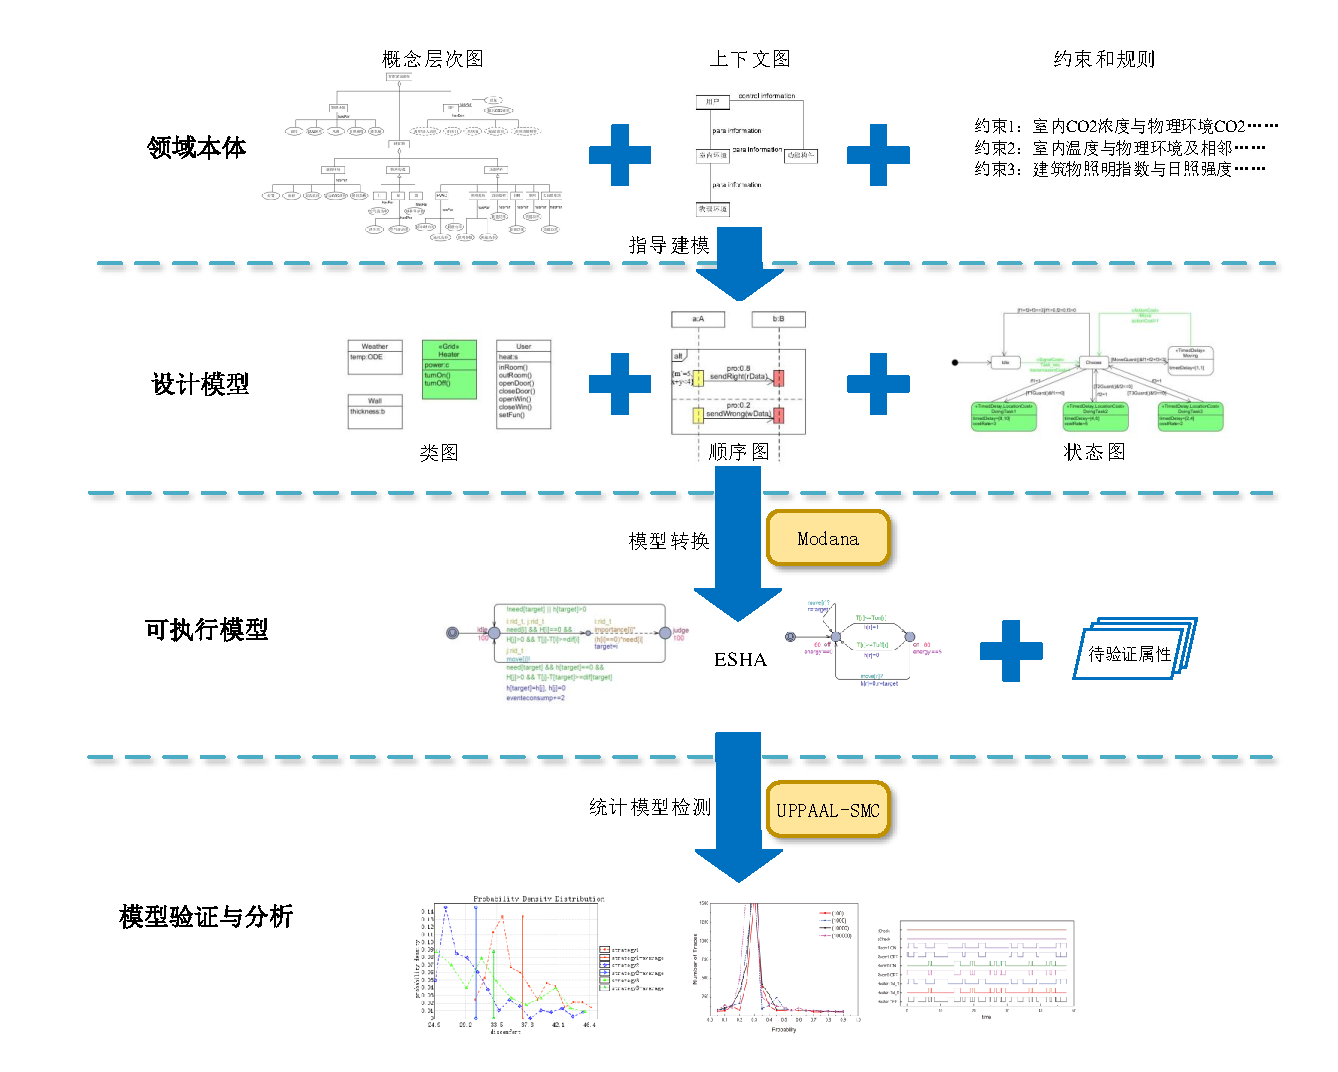
\includegraphics[width=6in]{framework.pdf}
	\caption{智能建筑能耗建模与分析方法}
	\label{approach-framework}
	\end{figure}
	
	如图\ref{approach-framework}所示,本文的主要贡献包括:	
	\begin{enumerate}
	\item 基于建筑信息模型和本体构造方法的基本步骤,给出了智能建筑的领域本体,帮助明确系统中的概念及概念间的关系和约束,指导建模系统的初步模型;
	\item 针对如何建模、描述CPES系统的问题,扩展了MARTE/UML的基本元素,以及类图、顺序图和状态图的元模型,以支持能耗、随机和混成的建模;
	\item 针对如何评估、分析CPES系统能耗的问题,定义了能耗随机混成自动机的概念,并给出从MARTE/UML状态图到能耗随机混成自动机的转换规则和算法。基于我们的Modana工具和模型验证工具UPPAAL-SMC,给出了本文所提的建模、分析方法的实现框架;
	\end{enumerate}
	
	此外,结合一个具体的智能温控系统场景,我们实现了该系统的领域本体指导建模初步模型、模型设计和模型分析的全过程,验证了所提方法的可行性和有效性。
\section{本文组织结构}
	全文共包括六章,组织结构如下:
	
	第一章首先介绍了研究背景,即能量信息物理融合系统和智能建筑,其目前的研究现状以及研究热点。接着介绍了国内外对CPES和智能建筑进行系统建模、验证的相关工作,以及本文涉及到的相关理论与技术基础。最后总结了本文的主要工作与贡献,并给出了本文的组织结构。
	
	第二章将本体论的知识引入智能建筑能耗的建模与分析方法。首先,基于建筑信息模型和本体构造方法的基本步骤,给出了智能建筑的领域本体,包括智能建筑中的基本概念、概念间的关系和约束,接着,介绍了如何基于领域本体指导建模MARTE/UML初步模型。
	
	在根据系统需求明确了建模元素之后,第三章介绍了基于MARTE/UML建模语言的系统模型设计理论。针对CPES 的能耗感知、随机和混成特性,扩展了MARTE/UML建模语言:1)定义了两种典型的随机行为;2)扩展了MARTE 中的数据类型和表达式;3)扩展了UML 的类图、顺序图和状态图以支持对能耗、随机和混成的建模。
	
	由于MARTE/UML模型为不可执行模型,只能用于系统的设计,为了实现对系统模型中能耗等属性的分析和评估,在第四章,本文定义了能耗随机混成自动机的概念,可以显式建模系统中的能耗,并给出了从扩展的MARTE/UML状态图到能耗随机混成自动机的转换规则。最后,基于我们的Modana平台和模型验证工具UPPAAL-SMC,给出了本文所提的建模与分析方法的实现框架。
	
	第五章针对一个具体案例——智能温控系统,给出了领域本体指导建模初步模型、模型精化为MARTE/UML 模型、模型转换为ESHA模型和模型验证与分析的全过程。通过统计模型检测技术对系统属性进行验证,分析了不同的调度策略和用户行为模式对系统能耗的影响。
	%实验结果表明,本文提出的建模、验证方法不仅支持对智能建筑系统的完整建模,而且可以帮助分析系统的能耗与其他因素的关系。
	
	最后,总结了全文,并提出下一步工作的方向。